\input{chapter-header.tex}
% ===========================================================================
\chapter{State of the Art}
\chaplabel{background}
\minitoc
% ===========================================================================
\introduction
% ===========================================================================

This chapter presents the related work to this dissertation. With that in mind, we organize and classify the related work in two different axis \ie virtualization aspects and runtime manipulation. The reader would notice that some of the related works we present may fit into more than one of these axis. However, for the sake of clarity, we emphasize the aspects we believe will clarify the understanding of the rest of this thesis.

The first part of this chapter focuses on runtime manipulation of object-oriented applications. We first show related work that focus on the safe modification of language semantics at runtime. Then, we show how metacircular runtimes aim to have an unified language runtime to ease its modification. \gp{I should add some conclusion}

The second part of this chapter starts by presenting a brief introduction to virtualization, its terminology and moreover its usage. We find amongst those usages, that the \emph{co-existence} and \emph{control} of virtual technology may fit into the manipulation of runtimes.
Following, we dive into related work that implement and apply those two techniques, but not in the runtime manipulation scenario as we understand it.\gp{should add some conclusion}

This chapter finishes by presenting a detailed description of the problem statement and a final outlook of the upcoming chapters in the light of the found problems.


% ===========================================================================
\newpage
% ===========================================================================

\section{Modifying the Runtime}
\gp{should really expand this part and say why it is relevant}
Modifying a runtime system can be a cumbersome task. On one side, we recognize that virtual machines and the languages that run on top of then are very interrelated and interdependent software components. For example, a language must comply to the execution model provided by its \VM~(\eg a bytecode set or an object model), and the \VM may understand the language's internals to manipulate it~(\eg run it, optimize it or manage its memory).

On the other side, reflective runtimes have a circular dependency on themselves: they rely on the concept of causal connection\gp{this is actually only true for reflective architectures}. When we make a change in a reflective runtime, we should ensure these causal connections still hold at any point of the runtime's life. In case a causal connection is broken, the runtime may become unusable as there is no means for it to keep reflecting upon itself correctly.

The related work we present in this section presents two main topics of interest for us. First, we present those works that target the modification of a language's semantics by safe means~(\ie avoiding crashes). We follow by looking at the field of metacircular runtimes and \VMs, to study how they ease the modification of a runtime by means of simplifying the language-\VM relation for development.

\subsection{Modification of language semantics}

\subsubsection*{Tower of Interpreters Model}

The original model of reflection as defined by Smith~\cite{Smit82c} is based on meta-level interpretation. A program is interpreted by an interpreter, such interpreter is interpreted by a meta-interpreter and so on, possibly ad-infinitum. This leads to a tower of interpreters, where each floor defines the semantics of the program~(interpreter of application) it interprets~(Figure \ref{fig:tower_of_interpreters}).

\begin{figure}[ht]
\begin{center}
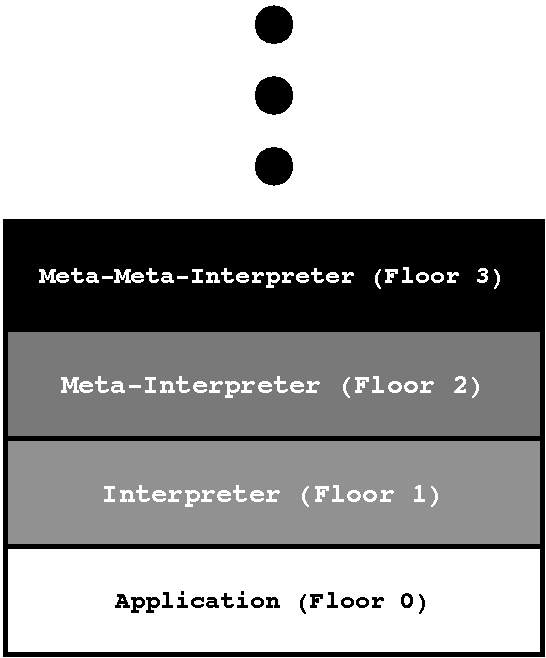
\includegraphics[width=.5\linewidth]{tower_of_interpreters}
\caption{\textbf{The theoretical tower of interpreters model. Each floor interprets the floor below itself.}\label{fig:tower_of_interpreters}
% (a)The host language and (b)the guest language contain each one their own classes and objects. The guest language resides inside the host language during the bootstrap; (c)the builder, a program written in the host language, reifies the bootstrap process itself and bootstraps the guest language given a (d)source code specification.
 }
\end{center}
\end{figure}

The tower of interpreters presents a model where one can define and redefine the semantics of the program it is executing. We can modify the behavior of our program~(in the floor zero) by jumping one level above it in the tower and modifying the interpreter running in that floor. In the same sense, we can jump one level above this interpreter to change also its behavior and so on. This allows the \emph{indirect modification} of a program's behavior \ie a change in an interpreter in a level \emph{n} changes the behavior of the interpreter level \emph{n - 1}, which impacts in the interpreter below it and so on, up to the base level.

Smith's tower of interpreters model is flexible and coherent regarding the manipulation of the reflective behavior of a program. The tower does not present a limit on the amount of interpreters we can stack, presenting a problematic infinite potential. This idea collides with the non-infinite amount resources in current machines. On one side, limited memory prevents us to have a tower of infinite interpreters running at the same time. On the other side, above certain limit of interpreters, this approach becomes too slow and impractical. We will show in the following subsections other reflective models that try to overcome these deficiencies while trying to keep some of the good properties of this model.

\subsubsection*{Black}

Black is a reflective language based on Scheme that mimics the infinite tower of interpreters with the goal to make it practical. Its model is based on the same idea as the reflective tower: the base level is interpreted by an interpreter, which is interpreted by a meta-interpreter and so on. The main difference between the original tower of interpreters and the model presented by Black is that the latter avoids the infinite regression, making the model practical in finite resource machines.

Black avoids the infinite regression by limiting the real levels of interpretation: there is only one level of interpretation. For the rest of the levels, Black  introduces a difference between directly-executed code in contrast with interpreted code. Directly-executed code is code that is executed by the machine, where no interpretation steps are involved. Then, the base-level application is the only interpreted code in the application. The rest of the tower, including the first interpreter, is implemented and executed directly in machine code~(Figure \ref{fig:black_tower}).

\begin{figure}[ht]
\begin{center}
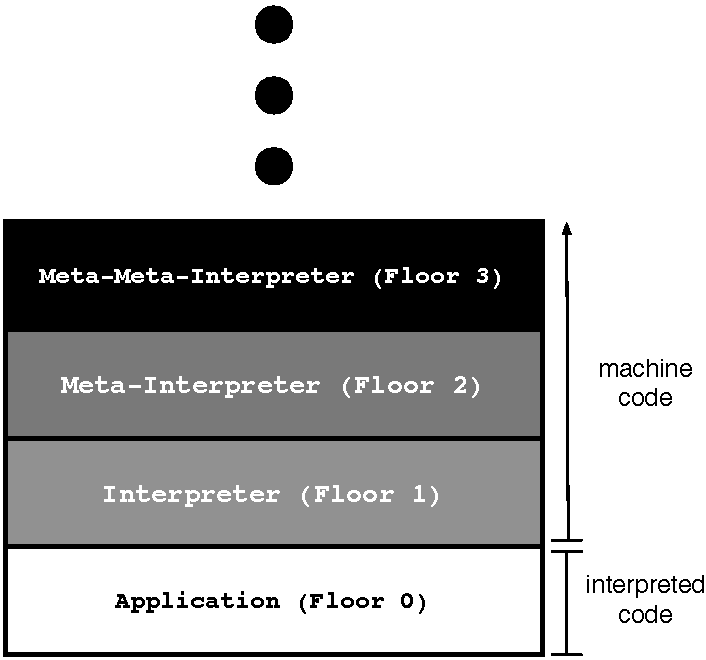
\includegraphics[width=.6\linewidth]{black_tower}
\caption{\textbf{Black.}\label{fig:black_tower}
% (a)The host language and (b)the guest language contain each one their own classes and objects. The guest language resides inside the host language during the bootstrap; (c)the builder, a program written in the host language, reifies the bootstrap process itself and bootstraps the guest language given a (d)source code specification.
 }
\end{center}
\end{figure}

By limiting the levels of interpretation, the model presented by Black forbids \emph{indirect modification}. Changing the interpreter in a level \emph{n} above the first level does not impact any more the interpreters below it, as they are directly-executed in the machine and not by the modified interpreter. Black supports, however, the modification of the first level of interpretation with the introduction of hooks inside the machine code. A hook detects wether a function in the interpreter~(written in directly-executed code) is changed, and interprets it by a meta-level interpreter written also in directly executed code. Hooks degrade the performance in comparison of a non-hooked interpreter, but it allows in exchange to change and specialize the behavior of the directly-executed code.

\subsubsection*{Safe-Tcl}
Safe-Tcl~\cite{Levy97a, Bore94a} is a variation of Tcl whose main purpose is the execution of Tcl scripts in a safe environment, with restricted permissions and attributions. Safe-Tcl achieves this by using \emph{twin interpreters} \ie a normal Tcl interpreter~(the master interpreter) can invoke and configure specialized interpreters that run isolated from the master interpreter~(Figure \ref{fig:safetcl_twin_interpreters}).

\begin{figure}[ht]
\begin{center}
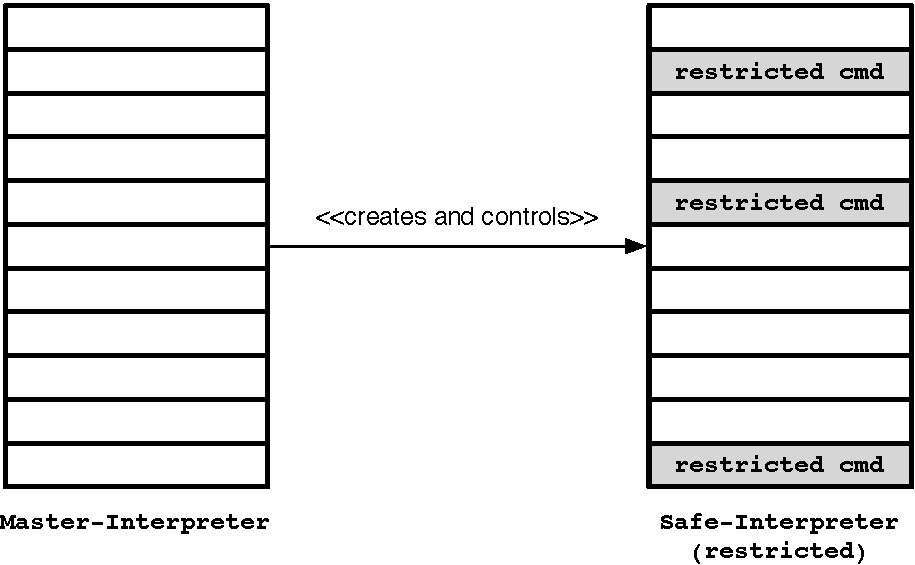
\includegraphics[width=.6\linewidth]{safetcl_twin_interpreters}
\caption{\textbf{Black.}\label{fig:safetcl_twin_interpreters}
% (a)The host language and (b)the guest language contain each one their own classes and objects. The guest language resides inside the host language during the bootstrap; (c)the builder, a program written in the host language, reifies the bootstrap process itself and bootstraps the guest language given a (d)source code specification.
 }
\end{center}
\end{figure}

The master interpreter modifies the behavior of a safe interpreter by providing a security policy. A security policy grants or removes privileges to the scripts executed on an interpreter. Commands can be aliased so the untrusted interpreter call an aliased method and the command is fully implemented by a trusted interpreter.

Safe-Tcl twin interpretation allows us to change the behavior of a program running on a specialized interpreter, without the limitations of the infinite tower of interpreters. However, in contrast with the solutions we already presented, Safe-Tcl does not provide with the ability to change completely the semantics of the language but just to override or provide new commands, with a focus on security.

\subsection*{Reflective Architectures and Reflectivity}

To enable reflection in mainstream languages such as Java, Ruby or JavaScript, the tower of interpreters is replaced by a reflective architecture~\cite{Maes87a}. Instead of relying on a stack of interpreters interpreting each the level below it, a reflective architecture relies on the idea of \emph{causal connection} \ie the programming language incorporates structures that represents aspects of itself~(\eg classes, objects), in such a way that if one structure changes the aspect it represents is updated accordingly, and vice-versa.


In languages presenting reflective architectures, reflection is controlled by a meta-object that lives in the same environment of the object it reflects upon.
One problematic corollary of this is that meta-objects rely on the same code and infrastructure than the objects they reflect upon; therefore there is a risk of infinite meta-recursion when the meta-level instruments code that it relies upon~(Figure \ref{fig:reflectivity_meta_recursion}).

\begin{figure}[ht]
\begin{center}
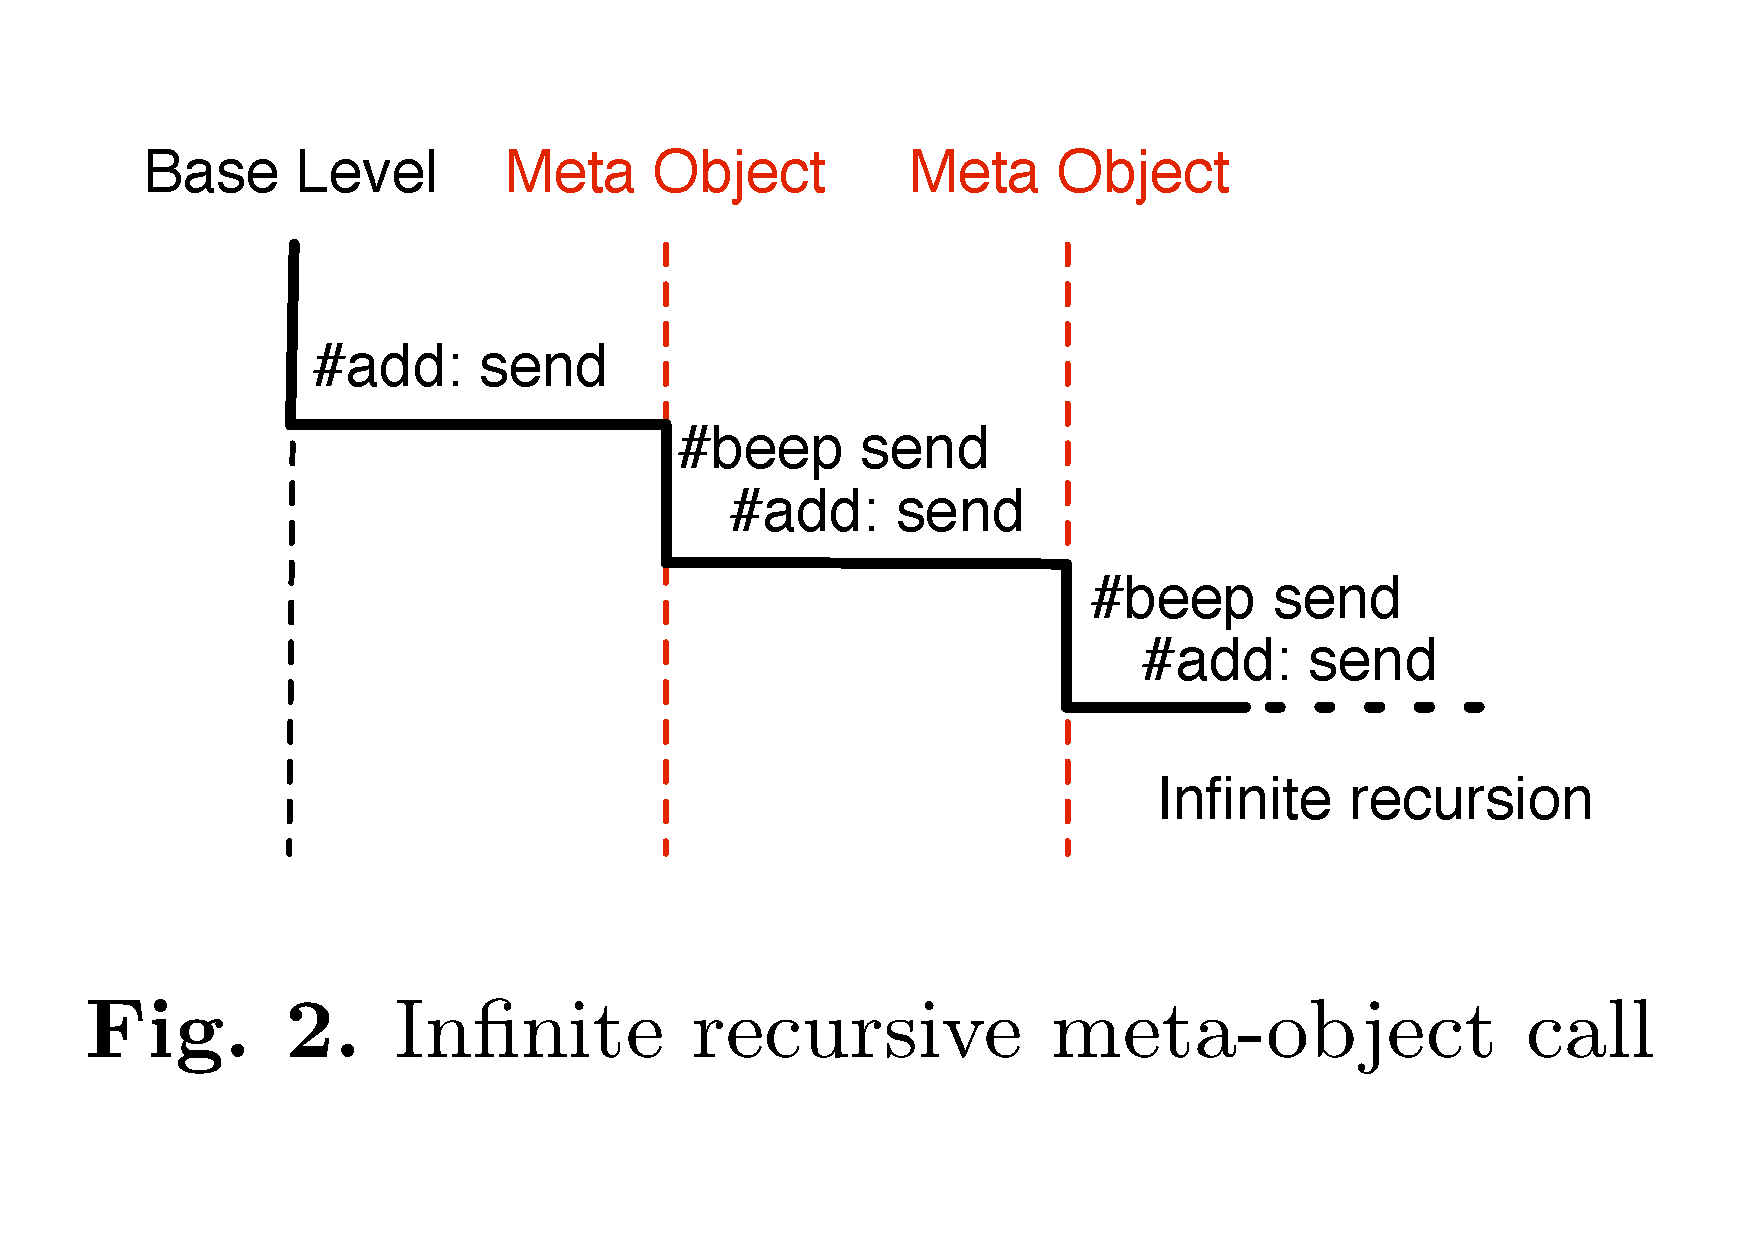
\includegraphics[width=.6\linewidth]{reflectivity_meta_recursion}
\caption{\textbf{Meta level recursion in reflective architectures.}\label{fig:reflectivity_meta_recursion}
% (a)The host language and (b)the guest language contain each one their own classes and objects. The guest language resides inside the host language during the bootstrap; (c)the builder, a program written in the host language, reifies the bootstrap process itself and bootstraps the guest language given a (d)source code specification.
 }
\end{center}
\end{figure}

Denker et al. solve this problem in Reflectivity~\cite{Denk08b}. Reflectivity is a reflective framework that avoids meta-recursions by tracking the degree of metaness of the execution context. In each reflective call, the \ct{MetaContext} object is activated and it accounts the meta-level jump. Likewise, when the reflective call returns, the \ct{MetaContext} is deactivated. Using the accounted meta-level jumps of the \ct{MetaContext}, meta-objects do only reflect on objects of a lower metaness~(and not greater or equal metaness). Thus, it simulates the semantics of an infinite tower of distinct interpreters while there is only one of them~(Figure \ref{fig:reflectivity_meta_recursion}).

\begin{figure}[ht]
\begin{center}
\begin{subfigure}{.45\textwidth}
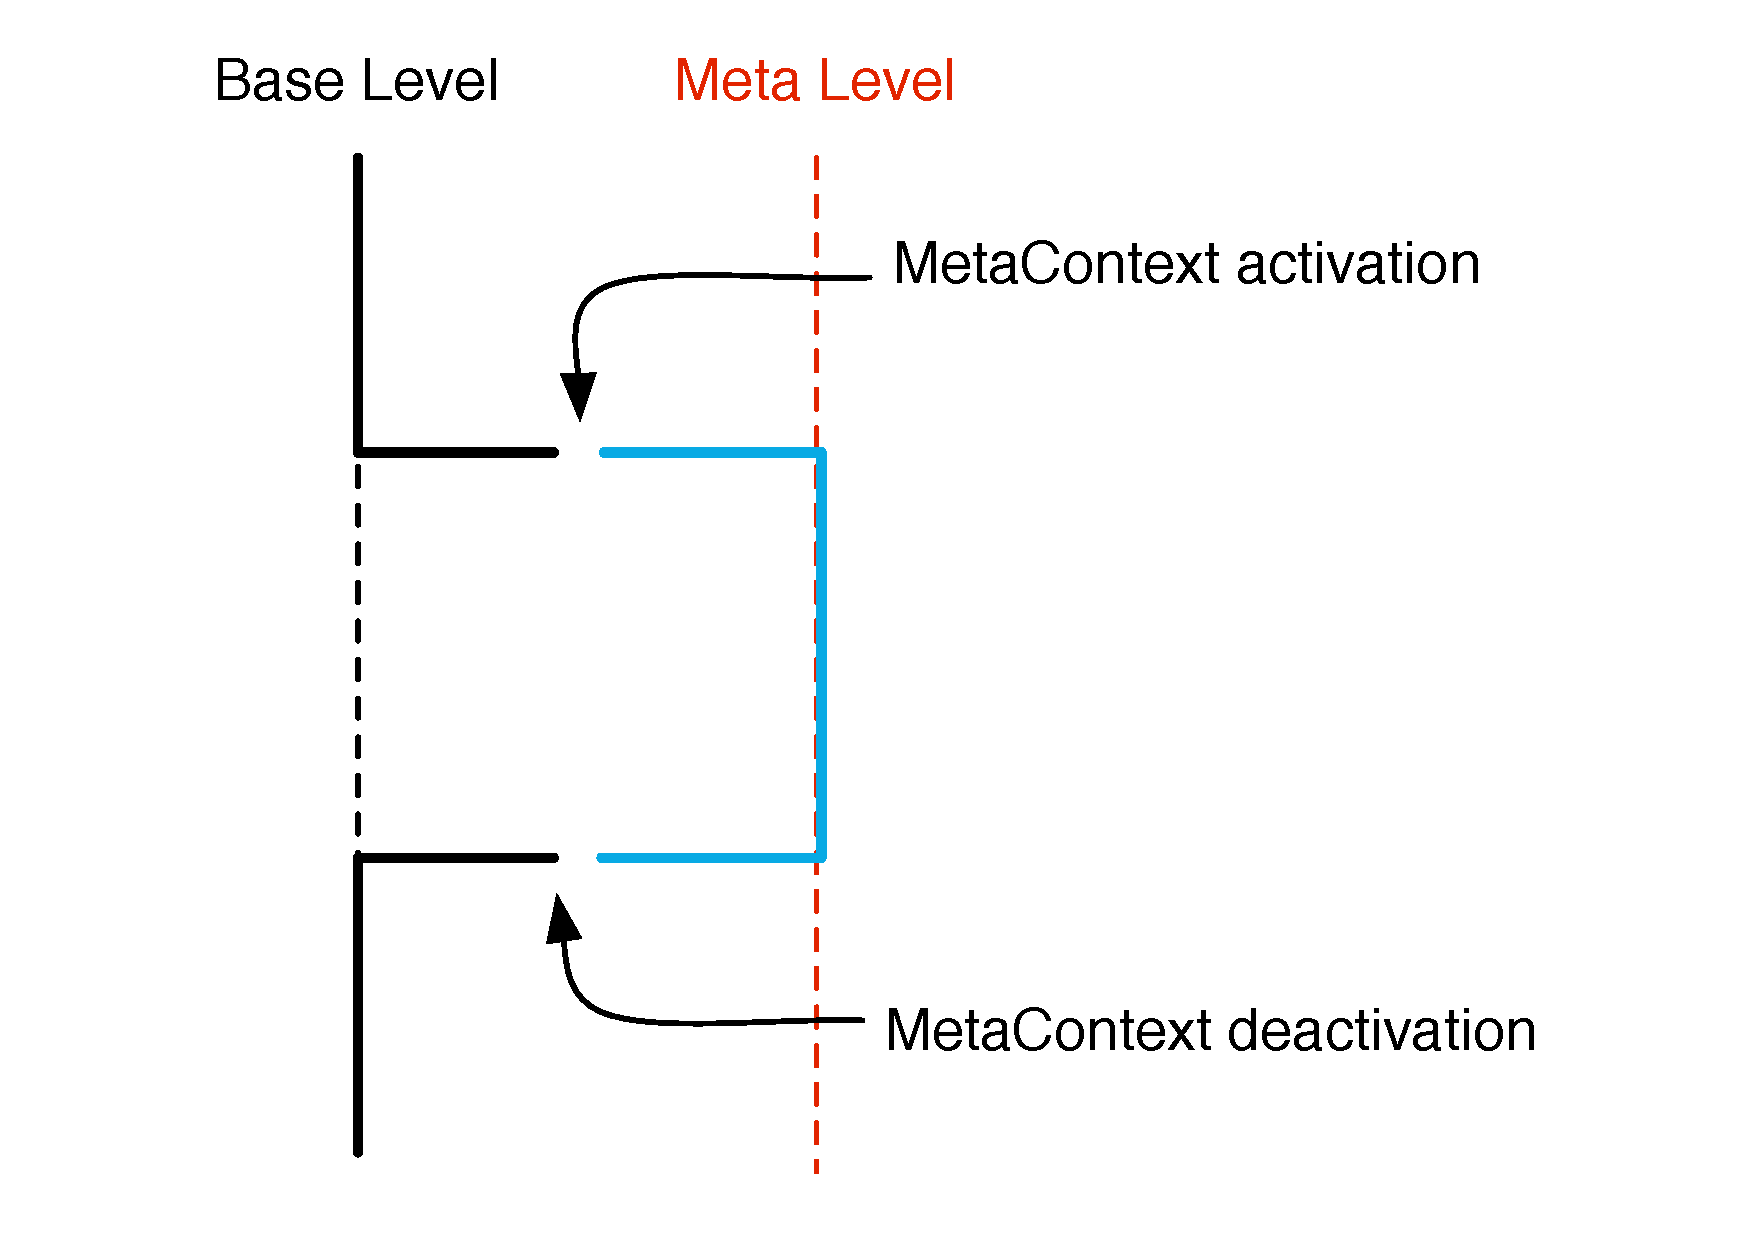
\includegraphics[width=1\linewidth]{reflectivity_metaness_accounting}
\end{subfigure}
\begin{subfigure}{.45\textwidth}
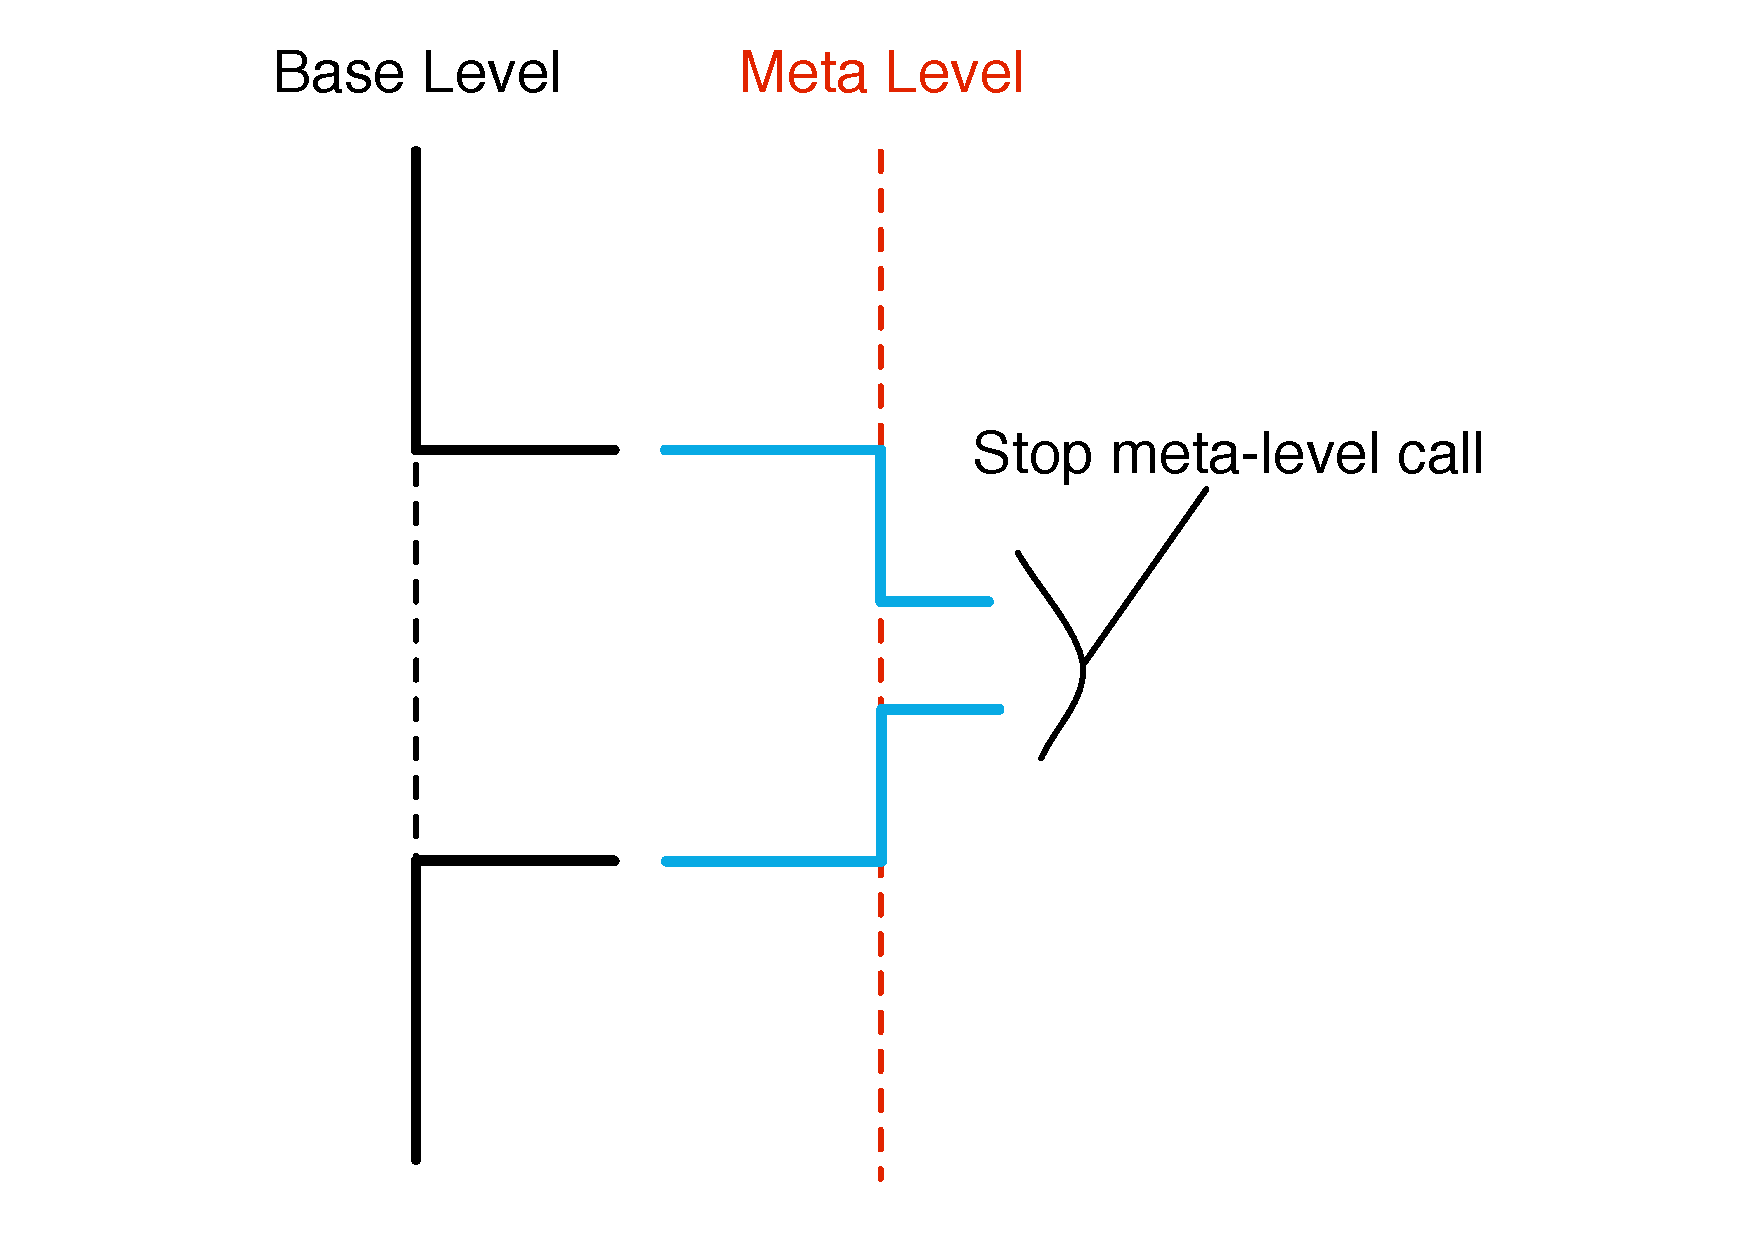
\includegraphics[width=1\linewidth]{reflectivity_avoid_recursion}
\end{subfigure}
\caption{\textbf{Meta level jump using reflectivity.}\label{fig:reflectivity_meta_recursion}
% (a)The host language and (b)the guest language contain each one their own classes and objects. The guest language resides inside the host language during the bootstrap; (c)the builder, a program written in the host language, reifies the bootstrap process itself and bootstraps the guest language given a (d)source code specification.
 }
\end{center}
\end{figure}

Reflectivity succeeds to modify and scope behavioral changes for different meta-levels inside the same reflective architecture. However, it does not provide with support for structural changes of the code the reflective framework depends upon.

\subsection{Metacircular Runtimes}

High-level language \VMs are inherent complex pieces of software.
They have to combine two rather extreme goals: abstraction and performance.
We have seen that the required abstraction for the running high-level language has a strong influence on the \VM design.
At the same time the hard performance requirement requires precise interaction with the underlying hardware.
This goes even so far that specialized hardware is conceived to match the performance requirements~\cite{Unga84a,Stef84a,McGh98a,Clic05a}.

The early \VMs focused on interpreting an abstract instruction set (bytecodes).
The benefits are twofold.
On the one hand the bytecodes guarantee certain platform independence by abstracting away from the \CPU specific instruction set.
On the other hand bytecodes allow to encode complex operations into little space both serving the hard memory constraints of the hardware and simplifying the design of a compiler.
Obviously this abstraction gain comes at a cost and ever since the first \VMs were built research and industry strive to reduce the interpretation overhead.
An efficient way to improve performance is to use a just in time compiler (JIT) that dynamically generates native code from the bytecode~\cite{Deut84a}.
In this case the bytecode becomes an intermediate representation (IR) for a bigger compiler infrastructure.
However, JIT compilers are notoriously complex as they crosscut many \VM components.
At the same time they crosscut all abstraction layers; they have to access high-level information from the running bytecodes and manage native code at the same time.
Similar complexity applies to the automatic memory management present in most high-level language \VMs.
Garbage Collectors (GC) evolved from simple helpers to complex software artifacts that for instance support concurrent garbage collection~\cite{Clic05a}.

The increased complexity of the \VMs lead to more novel approaches on how to build \VMs.
\VMs are still build for a big part in C or C++ for performance reasons.
However, there are more high-level approaches that try to simplify creating \VMs by using building blocks~\cite{Geof10a}.
In the following sections we are shedding light on metacircular \VMs which are programmed in the same language they in the end support.


\subsubsection*{Squeak Smalltalk \VM}
\seclabel{background-squeak}
% ---------------------------------------------------------------------------
The Squeak \VM~\cite{Inga97a} is of importance in the context of this work.
Its core building system is still in active use for the \urlfootnote{Cog \VM}{http://www.mirandabanda.org/cogblog/} which extends Squeak with a JIT compiler.
The Cog \VM is used as default by the \urlfootnote{Pharo}{http://pharo.org/} programming language.
Squeak is built around a Smalltalk dialect called Slang that is exported to C to be compiled to the final \VM binary.
Additionally, the Slang sources can be interpreted to provide an interactive simulator of the \VM, including full graphical support.

Slang is limited to the functionality that can be expressed with standard C code.
Slang in this case is mostly a high-level C preprocessor.
Even though Slang basically has the same syntax as Smalltalk it is semantically constrained to expressions that can be resolved statically at compilation or code generation time and are compatible with C.
Hence Slang's semantics are closer to C's than to Smalltalk's.
Unlike later metacircular frameworks, Squeak uses little or no compile-time reflection to simplify the \VM designs.
However, class composition help structuring the sources.
Next to the Slang source which account for the biggest part of the interpreter code some operating system related code and plugins are written in C.
To facilitate the interaction with the pure C part Slang supports inline C expressions and type annotations.

A great achievement of the Squeak \VM is a simulator environment that enables programmers to interact dynamically with the running \VM sources.
The simulator is capable or running a complete Squeak Smalltalk image including graphical user interface.
This means that programmers can change the sources of the running \VM and see the immediate effects in the simulator.
The simulator itself works by setting up a byte array which servers as native memory.
Then the \VM sources written in Slang are interpreted by the \VM of the development environment.

% ---------------------------------------------------------------------------
\subsubsection*{\Jikes: High-level low-level Programming with \MMTK}
\seclabel{background-jikes}
% ---------------------------------------------------------------------------
Jikes (former Jalapeño) is an early metacircular research \VM for Java written in Java~\cite{Alpe00a}.
The Jikes \VM features several different garbage collectors and does not execute bytecodes but directly compiles to native code.
With metacircularity in mind Jikes does not resort to a low-level programming language such as C for these typically low-level \VM components.
Instead they are written in Java as well using a high-level low-level programming framework.

The Jikes \VM had performance as a major goal, hence direct unobstructed interaction with the low-level world is necessary using a specialized framework.
High-level low-level programming \cite{Fram09a} is mentioned the first time in the context of the Jikes \VM project.
The goal of high-level low-level programming is to provide high-level abstractions to simplify low-level programming.
Essentially this is the same motivation that drives the metacircular \VM community.

Frampton et al. present a high-level low-level framework packaged as \ttt{org.vmmagic}, which is used as a system interface for Jikes. This package introduces highly controlled low-level interaction in a statically type context.
In their framework, methods have to be annotated to enable the use of low-level functionality.
Additionally their framework is successfully used in a separate project, the memory management toolkit (\textsc{MMTK})~\cite{Blac04a} which is used independently in several other projects.


% ---------------------------------------------------------------------------
\subsubsection*{Maxine Java \VM}
\seclabel{background-maxine}
% ---------------------------------------------------------------------------
Maxine is a metacircular Java \VM~\cite{Wimm13a} focused on an efficient developer experience.
Typically \VM frameworks focus on abstraction at the code-level which should yield simpler code and thus help reducing development efforts.
However, in most situations the programmer is still forced to use existing unspecific tools for instance to debug the \VM.
In contrast to that, the Maxine \VM provides dedicated tools to interact with the \VM in development.
Maxine uses abstract and high-level representations of \VM-level concepts and consistently exposes them throughout the development process.
Inspectors at multiple abstraction levels are readily available while debugging, giving insights to the complete \VM state.
Maxine provides and excellent navigation for generated native code by providing links back to language-side objects as well as other native code and symbols.

Even though the Maxine projects follows an approach where reflection is only used at compile-time, the development tools themselves provide a live interaction with the running \VM artifact.
However, the \VM itself is not reflective as it is not directly built to reason about itself.
This means that when debugging the \VM it behaves almost like a living Smalltalk image where a complete interaction with the underlying system is possible.
We identify this as crucial, as most of the time is spent debugging, notably on inadequate tools like \ttt{gdb} due to lack of alternatives.
Hence having a specific debuggers and inspectors greatly improve the interaction with the \VM artifact.


\subsubsection*{\PyPy Toolchain}
\seclabel{background-pypy}
% ---------------------------------------------------------------------------
\urlfootnote{\PyPy}{http://pypy.org/} is a \Python-based high-level \VM framework \cite{Rigo06a}.
\PyPy's major focus lies on an efficient \Python interpreter.
However, it has been successfully used to build \VMs for other languages including \ST \cite{Bolz08a}.
Interpreters are written in a type-inferable subset of \Python called \RPython.
The underlying \PyPy infrastructure automatically provides memory management and \JIT compilation.
Instead of explicitly providing these features, a \VM developer hints certain information to the \PyPy framework to improve the generation of a \GC or \JIT.

\PyPy follows a different approach from the previously presented \VM generation frameworks.
For instance, in Squeak and \Jikes the final \VM implementation is not much different from an implementation done directly in a low-level language.
The programmer specifies all the components of the \VM explicitly, either by implementing them directly or using a provided library.
Compared to the more static C ans C++ these \VM generation frameworks make the compilation phase more tangible.
\ST in \Squeak or \Java in \Jikes or \Maxine fulfill the purpose of the template system in C++ or the restricted macro system in C.
For the explicit implementation part \PyPy is no different.
However, certain features for the final \VM are directly absorbed from the underlying \PyPy infrastructure.
For instance, the \JIT support or the \GC are not explicitly implemented but provided by the \PyPy framework itself.
This is a big difference to the other \VM frameworks as it allows programmers to write the \VM in a more high-level fashion.
For instance in \Squeak memory allocation, even for \VM-level objects, has to be performed explicitly.
Whereas in \PyPy the garbage collection is left to the underlying \VM building infrastructure.
This approach allows \RPython \VMs to behave like standard \Python programs.

Much like the automatic memory management, \PyPy provides a tracing \JIT generator \cite{Bolz09a}.
By default the \VM programmer does not write an explicit \JIT in \PyPy.
Instead the \VM code is annotated to guide the underlying tracing \JIT generator.
This means a \VM compilation time a specific tracing \JIT is created for the given meta information.
As a result, the \JIT can track high-level loops in the final interpreted language.
Again, this is similar to \PyPy's \GC, both are provided as a service and do not have to be programmed explicitly.
Instead, the \VM programmer tweaks parameters of the \JIT or \GC.

% ------------------------------------------------------------------------------
\subsubsection*{\Pinocchio \VM}
\seclabel{background-pinocchio}

\P \cite{Verw11a} is a research \ST environment that directly uses native code instead of bytecodes.
The only execution base is native code which is directly generated by the language-side compiler.

\P is built from a kernel derived originally from a \PH image.
For the bootstrap classes, objects and methods are exported into binary, native images and linked together with a standard C linker to a final executable.
For simplicity we also rely on a very small part of C code to provide essential primitive, for instance used for file handling.
Additionally we specified part of the bootstrap for the \ST object model in plain C code.
However, besides that, all the other code is written and developed directly in \ST.

An important aspect of \P is that the method lookup is expressed in terms of normal \ST code.
Typically this code statically resides in the \VM, thus at a different meta-level.
Hence this implies for most systems that the lookup can not be modified without altering the \VM itself.
However, expressing the lookup in terms for normal language-side code introduces a recursive dependencies during the bootstrap.
In order to run the lookup code expressed in \ST code, we have to perform message sends.
These, in return, require an already working lookup mechanism.
Hence, without a taking special care, a language-side lookup method will lead to infinite recursion during startup.
We resolved this problem in \P by directly interacting with the low-level execution format which among other things relies on inline caches to improve performance.
The important property of inline caches is that they bypass the slow language-side lookup by directly jumping to the last activated method at a send-site.
This is exactly the behavior we need to prevent recursion during the startup.
Hence, when generating the native code for the bootstrap, we prefill all the inline caches of the methods required to perform a full method lookup.
As a result, when running requiring the first real method lookup, the lookup code itself is running perfectly on the prefilled inline caches.
What we achieve is a flexible connection between the low-level world and the high-level language-side.
During execution the \VM jumps freely between what previously was native \VM-level code and interpretation of language-side code.

% ------------------------------------------------------------------------------
\subsubsection*{\Klein \VM}
\seclabel{background-klein}

\urlfootnote{\Klein}{http://kleinvm.sourceforge.net/} is a metacircular \VM for the \Self programming language that has no separation into \VM and language \cite{Unga05a}.
It is important to point out that the reification of the \VM-level survives the code generation or compilation time.
Instead the \VM structures are represented as real \Self objects.
Hence the \Klein \VM supports true \VM-level reflection since there is only a single code base.

Additionally to the advances in reflection and metacircularity, \Klein focuses on fast compilation turnarounds to allow for a responsive development process.
Which is unlike for instance the \Squeak \VM where a full \VM bootstrap takes an order of minutes on modern hardware.
\Klein also supports advanced mirror-based debugging tools to inspect and modify a remote \VM.

Development on the \Klein \VM stopped in 2009 and left the \Klein \VM in fairly usable state.
Like \P it currently lacks a dedicated \GC.
Yet, it proved that it is possible and build a language-runtime without the classical separation of the language-side and the \VM.
From the literature presented about the \Klein project we see a strong focus on the improvements of the development tools.
The fact that the language-runtime allows \VM-level reflection to change the \VM dynamically is not directly mentioned in the literature.
While we see the practical limitations of changing the \VM at runtime we would like to open the doors to this new form of reflection.

\section{Virtualization Techniques}

\gp{introduction}

\subsection{Application Co-existence}

\subsubsection*{\textsc{Class Loaders}}
In Java, classes are loaded dynamically through a class loader~\cite{Lian98a}. A class loader is a first-class entity responsible of loading classes: create their runtime representation, loading their methods and linking their class references. A class loader remembers all classes it loaded, and it is responsible for loading all classes related to  them. Class loaders define namespaces: different class loaders can load different classes with the same name. These classes will be isolated in the sense that they will not be visible to the others.

Class loaders can be specialized and extended to provide custom behavior. For example, Fong et. al.~\cite{Fong10a} use the class loading mechanism to enforce scoping rules and determine the visibility of names in various region of the program. They allow the user to control untrusted
namespaces and classes, they have defined a language to define security policy. Jensen et. al.~\cite{Jens98a} provide a formalization of the class loader with the means to enforce security. They also use a bytecode verifier on class loading to check if a class' bytecode doesn't try to perform overflow or underflow operations.

The isolating mechanism of class loaders is useful in the scoping context. New versions of code can be loaded in a different class loader and coexist at runtime. However, its basic mechanism does not support a way to manage changes, or update an application.

\subsubsection*{\textsc{Changeboxes}}

Changeboxes~\cite{Denk07c} is a change model designed to encapsulate and scope changes. Its main purpose is to allow several versions of a system to coexist at runtime \ie the existence in the same environment of different versions of the same classes and methods. In changeboxes, a \emph{changebox} is a first-class entity that encapsulates changes made on elements~(classes and methods) and an executable version of the system with its changes applied. The system can contain many changeboxes at the same time, and applications can be scoped to run within different changeboxes. This notion of dynamically scoping an application to a changebox allows one to have co-existing environments~(\eg testing, development, production), increasing the developer's efficiency. Furthermore, it eases application update and migration to new versions, and reduces its update down-time as the application does not have to be stopped to be updated.

A Changeboxes prototype was developed in Smalltalk and its scoping mechanisms were implemented as follows:

\begin{description}
\item[Message send interception.] Message sends can activate different methods, within different changeboxes. A MethodWrapper~\cite{Bran98a} is placed instead of the method that has multiple versions, and it delegates the execution to the method that corresponds to the currently valid changebox.

\item[Class access interception.] Smalltalk resolves class names at compile time, inserting a reference to the given class inside the method's literal array. However, accessing a class should yield different class objects if the changebox contains a different version of it. To resolve this, class accesses affected by a changebox are postponed until runtime, and the code is recompiled in such a way: instead of putting the class inside the literal array, the class is dynamically looked-up from the class table when it is accessed.
\end{description}

Changeboxes model proves sound to update and migrate application and framework classes. However, it has the main drawback of not affecting critical classes in the system. Changeboxes prototype does not work on classes such as \ct{Array} or \ct{CompiledMethod} as the underlying infrastructure~(the VM) restricts the system to the existence of only one of them at the same time. The changes model does not provide neither a solution for this problem, as it focuses on application code update, leaving this as an open problem.

\subsubsection*{\textsc{Caja\textbackslash Cajita}}

\subsubsection*{\textsc{Worlds}}
Worlds~\cite{Wart08a} provide a way to control and scope side-effects in Javascript. Side-effects are limited to a first-class environment.

\subsubsection*{\textsc{Gemstone}}
Gemstone \cite{Otis91a} provides the concept of class versions. Classes are
automatically versioned, but existing instances keep the class (shape and
behavior) of the original definition. Instances can be migrated at any time.
Gemstone provides (database) transaction semantics, thus state can be rolled
back should the migration fail.
Gemstone's class versions extend the usual Smalltalk class evolution mechanism for robustness, 
large datasets, and domain-specific migration policies. In contrast, ObjectSpaces target general 
reflective access and bootstrap-like evolutions of code that is critical to the environment.

\subsubsection*{KaffeOS}
KaffeOS \cite{Back00a} makes an explicit domain separation in memory by using different memory heaps in the virtual machine. They enforce domain separation by using memory write barriers. Cross-domain references become cross-heap references, and thus, they need special virtual machine support.
KaffeOS presents a model where resource accounting is handled at the level of the virtual machine.

\subsubsection*{J-Kernel}
J-Kernel \cite{Hawb98a}

\subsubsection*{Luna}
 and Luna \cite{Hawb02a} present a solution similar to ours regarding the memory usage. They are Java solution for isolating object graphs with security purposes. In them, each object graph is called a \emph{protection domain}. All protection domains loaded in a system, and their objects, share the same memory space. 

The J-Kernel enforces the separation between domains by using the Java type system, the inability of the Java language to forge object references, and by providing capability objects\cite{Levy84a,Mill03a,Spoo00a} enabling remote messaging and controlling the communication. This same separation in Luna \cite{Hawb02a} is achieved by the modification of the type system and the addition in the virtual machine of the \emph{remote reference} concept.

\subsection{Application Control}

\subsubsection*{JVMTI}
Java also provides JPDA, a remote debugging architecture that specifies a native interface on the debuggee VM, and a matching API for the debugger front-end, running in a separate VM. However, JDPA only supports introspection features like  inspection and monitoring, and very limited intercession \cite{jdpa}.

\subsection*{Xen and Operating System Virtualization techniques}
Amongst the most important works on virtualization,we can found approaches like Xen~\cite{Chis07xen}. Xen is a Virtual Machine Monitor~(VMM) that allows to control and manage Virtual Machines in a high performance and resource-managed way. This approach targets the virtualization of full and unmodified operating systems, to facilitate their adoption in industrial/productive environments. Virtualization, in these terms, enables the following applications:

\begin{description}

\item[Server Consolidation.]
\item[Co-located hosting facilities.]
\item[Distributed web services.]
\item[Secure computing platforms.]
\item[Application Mobility.]

\end{description}

This virtualization approach has another main characteristic: it considers its guest systems as a black box, and it does not allow one to observe or modify its internals.

\subsubsection*{MVM: a Multi User Virtual Machine}
The Multi-user Virtual Machine~\cite{Czaj03a,Czaj01a} is a general purpose virtual machine for the Java language that allows the co-existence of different applications, potentially from different users. Each application running on top of the MVM is an \emph{isolate} based on the Java Application Isolation API specification~\cite{JSR121}.

Many isolates co-exist not inteferring each other, as they believe they own their private JVM: the runtime is modified, so state is not shared between them by default. MVM allows several communication mechanisms to securely communicate isolates: from standard mechanisms such as sockets, up to \emph{links}, a low-level isolate-to-isolate mechanism introduced by the Isolate API.

MVM can run any normal Java application. Additionally, MVM-aware applications can use the API it provides to control the life-cycle~(\eg creation, suspension, resuming and and termination) and the available resources of other isolates.

%\subsection*{Java Isolates}
%Java Isolates \cite{JSR121} allow multiple applications to run inside the same Java virtual machine.
%Nothing is shared between the different applications. Resources like CPU time, memory are controlled 
%and restricted. Isolates can communicate through channel, since nothing is shared the data are copied. 
%Java Isolates are defined in the Java Specification Request 121, but no commercials Java virtual 
%machine implement the specification.

\section{Problem Statement}

% =============================================================================
\input{chapter-footer.tex}